\begin{figure}[H]
  \centering

  \tikzset{
    pics/cell/.style={
      code={
        \draw (-0.25,-0.25) rectangle (0.25,0.25);
        \fill (0,0) circle(0.05);
        \draw[->] (0,0) -- (#1-0.25, 0);
      }
    }
  }
  \tikzset{
    pics/nil/.style={
      code={
        \draw (-0.25,-0.25) rectangle (0.25,0.25);
        \fill (0,0) circle(0.05);
      }
    }
  }

  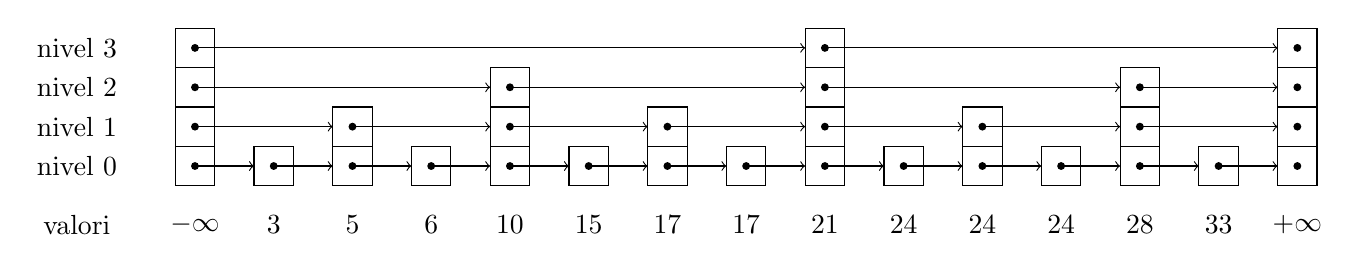
\begin{tikzpicture}
    \foreach \x in {0,...,13} {
      \draw (\x,0) pic{cell={1}};
    }
    \draw (14,0) pic{nil};

    \foreach \x in {0,2,...,12} {
      \draw (\x,0.5) pic{cell={2}};
    }
    \draw (14,0.5) pic{nil};

    \draw (0,1) pic{cell={4}};
    \draw (4,1) pic{cell={4}};
    \draw (8,1) pic{cell={4}};
    \draw (12,1) pic{cell={2}};
    \draw (14,1) pic{nil};

    \draw (0,1.5) pic{cell={8}};
    \draw (8,1.5) pic{cell={6}};
    \draw (14,1.5) pic{nil};

    \begin{scope}[shift={(0,-0.75)}]
      \node at (0, 0) {$-\infty$};
      \node at (1, 0) {$3$};
      \node at (2, 0) {$5$};
      \node at (3, 0) {$6$};
      \node at (4, 0) {$10$};
      \node at (5, 0) {$15$};
      \node at (6, 0) {$17$};
      \node at (7, 0) {$17$};
      \node at (8, 0) {$21$};
      \node at (9, 0) {$24$};
      \node at (10, 0) {$24$};
      \node at (11, 0) {$24$};
      \node at (12, 0) {$28$};
      \node at (13, 0) {$33$};
      \node at (14, 0) {$+\infty$};
    \end{scope}

    \node at (-1.5,0) {nivel 0};
    \node at (-1.5,0.5) {nivel 1};
    \node at (-1.5,1) {nivel 2};
    \node at (-1.5,1.5) {nivel 3};
    \node at (-1.5,-0.75) {valori};

  \end{tikzpicture}

  \caption{O listă pe niveluri, utilă pentru date statice.}
  \label{fig:skip-lists-static}
\end{figure}
